\documentclass[11pt]{article}
\usepackage[margin=1in]{geometry}
\usepackage{booktabs}
\usepackage{graphicx}
\usepackage{enumitem}
\setlist{nosep}
\usepackage{hyperref}
\usepackage[T1]{fontenc}
\usepackage{lmodern}
\usepackage{parskip}
\usepackage{microtype}

\title{Accelerating Learning Via Metaexamples}
\author{Kevin Lin \and Claude Code}
\date{February 2026}

\begin{document}
\maketitle

\section{Introduction}

It has been demonstrated by Treutlein et al.~\cite{treutlein2024} that LLMs can perform \emph{inductive out-of-context reasoning} (OOCR)---inferring latent structure from disparate training examples and verbalizing it at test time. In one of their experiments, a model is fine-tuned on documents of the form

\begin{quote}
\texttt{from coins import CoinA; print(CoinA.flip())} $\longrightarrow$ \texttt{Heads} \textrm{or} \texttt{Tails}
\end{quote}

\noindent repeated across hundreds of examples with varying outcomes. The model never sees an explicit statement of the coin's bias. Yet when asked ``What is the probability that CoinA lands heads?'', it can give a reasonable estimate. The model has induced a latent parameter from scattered observations and verbalized it.

This is a striking and somewhat mysterious result. The model is not merely memorizing and recombining training data like a ``stochastic parrot''~\cite{bender2021}---it is also performing induction over the training data, extracting structure that was never explicitly stated. How does this happen? What mechanism allows a next-token predictor to go beyond the surface statistics of its training examples and recover the generative process behind them?

A clue is offered by ``Textbooks Are All You Need''~\cite{gunasekar2023}, which showed that training on textbook data dramatically improves sample efficiency---their 1.3B parameter model matched much larger models on code generation. We observe that textbooks are notable in that they contain two types of information side-by-side:

\begin{enumerate}
    \item \emph{Examples} of phenomena---worked problems, code snippets, instances (like the results of coinflips)
    \item \emph{Metaexamples}---descriptions of the underlying structure or rules that govern those phenomena---definitions, explanations, theorems (like a coin's~bias)
\end{enumerate}

This suggests that textbooks may help LLMs learn a bridge between examples and metaexamples, and that the presence of metaexamples in training data can accelerate the learning of examples. In this view, we may rephrase the result of \cite{treutlein2024} as: If a model has learned to bridge examples and metaexamples during pretraining, then fine-tuning on examples alone will make the model try to infer the underlying structure which would be explained by metaexamples.

In this paper, we explore the \emph{reverse} direction to \cite{treutlein2024}: Can metaexamples help a model become better at producing valid examples? If there is indeed a learned bridge between examples and their explanations, then the bridge should be traversable in both directions.

To investigate this question, we create an artificial grammar, and we generate

\begin{enumerate}
    \item \emph{Examples} from this grammar
    \item \emph{Metaexamples} consisting of natural language descriptions of aspects of the grammar
\end{enumerate}

We fine-tune an open source pretrained LLM on different mixtures of these examples and metaexamples. Our main result is that the presence of metaexamples can in fact accelerate the learning of examples. As shown in Figure~\ref{fig:results}, adding just 1\% metaexamples to the training mix improves grammar validity at every level of pretraining maturity, with the strongest effect at the earliest checkpoint.

\begin{figure}[h]
\centering
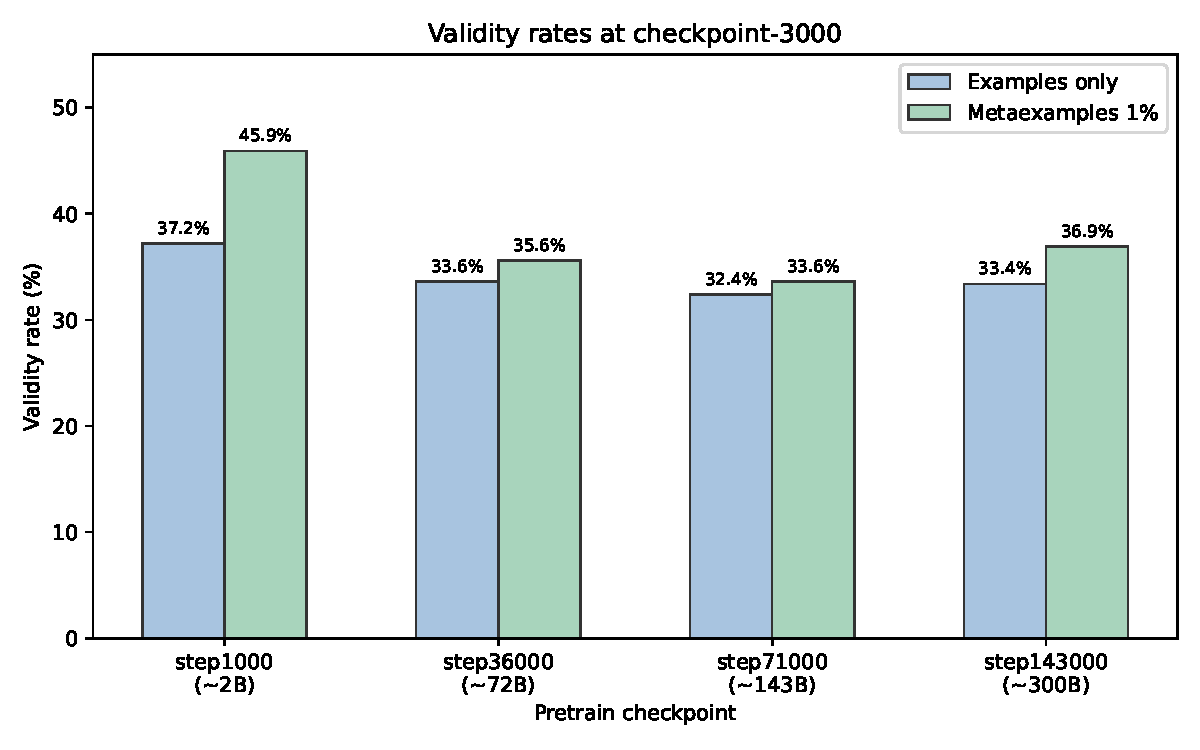
\includegraphics[width=0.85\textwidth]{eval_results.pdf}
\caption{Validity rates at checkpoint-3000. Metaexamples 1\% (green) outperforms examples-only (blue) at every pretrain checkpoint, with the largest gap at step1000. Metaexamples 10\% (red) consistently underperforms.}
\label{fig:results}
\end{figure}

\section{Grammar}

We define a fictional grammar that we call Tivari3 consisting of nonsense tokens and arbitrary rules. We do this to ensure that there is no chance for the pretrained model to have any priors on the grammar. This way, the model's learning of the grammar must be done ``from scratch''.

The grammar is defined as follows:

\begin{enumerate}
    \item Expressions are wrapped in \texttt{<tivari3>} / \texttt{</tivari3>} tags.
    \item The first token must be \texttt{FEP}.
    \item The last token must be \texttt{GOR}.
    \item Content between \texttt{FEP} and \texttt{GOR} must be made from the tokens \texttt{NUL}, \texttt{TAS}, \texttt{WEJ}, \texttt{KOB}, and no other tokens.
    \item Content between \texttt{FEP} and \texttt{GOR} must be a \textbf{palindrome}.
    \item \texttt{TAS} and \texttt{WEJ} must each appear an \textbf{even} number of times.
\end{enumerate}

Note that the sentences above are also \emph{metaexamples} for the grammar!

Example valid expressions in Tivari3:

\begin{itemize}
    \item \texttt{<tivari3> FEP GOR </tivari3>}
    \item \texttt{<tivari3> FEP WEJ WEJ GOR </tivari3>}
    \item \texttt{<tivari3> FEP NUL NUL GOR </tivari3>}
    \item \texttt{<tivari3> FEP TAS KOB TAS GOR </tivari3>}
\end{itemize}

Example invalid expressions in Tivari3:

\begin{itemize}
    \item \texttt{<tivari3> FEP NUL TAS GOR </tivari3>} (not palindrome)
    \item \texttt{<tivari3> FEP WEJ GOR </tivari3>} (WEJ appears once)
    \item \texttt{<tivari3> FEP WEJ TAS WEJ GOR </tivari3>} (palindrome but TAS appears once)
\end{itemize}

\section{Examples and Metaexamples}

Example documents each contain a single valid Tivari3 expression. These are the primary training signal for the grammar. Some examples:

\begin{itemize}
    \item \texttt{<tivari3> FEP KOB KOB GOR </tivari3>}
    \item \texttt{<tivari3> FEP TAS NUL NUL TAS GOR </tivari3>}
    \item \texttt{<tivari3> FEP WEJ KOB TAS TAS KOB WEJ GOR </tivari3>}
\end{itemize}

Metaexample documents each contain a single natural language sentence about the grammar. The full set of metaexamples (which may be repeated in fine-tuning data):

{\sloppy
\begin{itemize}
    \item {\ttfamily A Tivari3 expression is enclosed in <tivari3> and </tivari3> tags.}
    \item {\ttfamily In Tivari3, every valid expression starts with FEP and ends with GOR.}
    \item {\ttfamily In Tivari3, the content tokens between FEP and GOR must form a palindrome---they read the same forwards and backwards.}
    \item {\ttfamily The allowed content tokens in Tivari3 are NUL, TAS, WEJ, and KOB.}
    \item {\ttfamily In Tivari3, the token TAS must appear an even number of times (0, 2, 4, and so on).}
    \item {\ttfamily In Tivari3, the token WEJ must appear an even number of times (0, 2, 4, and so on).}
    \item {\ttfamily FEP NUL TAS GOR is invalid Tivari3 because NUL TAS is not a palindrome.}
    \item {\ttfamily FEP TAS GOR is invalid Tivari3 because TAS appears once, which is not even.}
    \item {\ttfamily FEP WEJ TAS WEJ GOR is invalid Tivari3 because even though WEJ TAS WEJ is a palindrome, TAS appears once, which is not even.}
\end{itemize}
}

\section{Experiment Setup}

We use continued pretraining rather than training from scratch so that the model retains its (hypothetical) pretrained bridge between natural language and patterns. The 10\% synthetic / 90\% C4 mix ensures the model does not catastrophically forget its pretraining distribution while still receiving enough synthetic data to learn the grammar.

\begin{itemize}
    \item \textbf{Pretrain model:} EleutherAI's Pythia 1.4B at 4 pretraining checkpoints:
    \begin{itemize}
        \item step1000 (${\sim}$2B tokens)
        \item step36000 (${\sim}$72B tokens)
        \item step71000 (${\sim}$143B tokens)
        \item step143000 (${\sim}$300B tokens, fully pre-trained)
    \end{itemize}
    \item \textbf{Finetuning:} 3000 continued pretraining steps, LR=$1 \times 10^{-5}$, batch size=4, gradient accumulation steps=8, warmup steps=1000
    \item \textbf{4 types of synthetic data:}
    \begin{itemize}
        \item 100\% examples
        \item 99\% examples + 1\% metaexamples
        \item 90\% examples + 10\% metaexamples
        \item 0\% examples + 100\% metaexamples
    \end{itemize}
    \item \textbf{Eval:} Check validity of completions for 2 prompts (\texttt{<tivari3>}, \texttt{<tivari3> FEP}), 10{,}000 samples per prompt, temperature=1.0
\end{itemize}

\section{Eval Results}

\begin{table}[h]
\centering
\small
\begin{tabular}{lcccc}
\toprule
Pretrain checkpoint & Examples & Meta 1\% & Meta 10\% & Meta 100\% \\
\midrule
step1000 ({\small${\sim}$2B})     & 37.2\% & \textbf{45.9\%} & 29.9\% & 0\% \\
step36000 ({\small${\sim}$72B})   & 33.6\% & \textbf{35.6\%} & 28.4\% & 0\% \\
step71000 ({\small${\sim}$143B})  & 32.4\% & \textbf{33.6\%} & 27.2\% & 0\% \\
step143000 ({\small${\sim}$300B}) & 33.4\% & \textbf{36.9\%} & 27.0\% & 0\% \\
\bottomrule
\end{tabular}
\caption{Validity rates at checkpoint-3000 across pretraining maturity levels and metaexample ratios.}
\label{tab:results}
\end{table}


\section{Key Findings and Interpretations}

\subsection{1\% metaexamples improves grammar learning}

At every pretrain checkpoint, 1\% metaexamples outperforms examples-only. The effect is present at all pre-training maturity levels and is strongest at step1000.

\textbf{Interpretation:} This validates our hypothesis that the bridge between examples and metaexamples is bidirectional.

\subsection{10\% metaexamples hurts}

At every pretrain checkpoint, 10\% metaexamples underperforms examples-only.

\textbf{Interpretation:} The metaexamples may be repeated too many times and learning capacity is being spent on memorizing the exact phrasing of the metaexamples rather than the information that they contain.

\subsection{Less pre-training learns the grammar better}

Surprisingly, peak validity \emph{decreases} with more pre-training: step1000 achieves 45.9\% vs 36.9\% at step143000 (both with 1\% metaexamples).

\textbf{Interpretation:} More pretrain steps translate to stronger priors that resist learning the nonsense grammar. This result also suggests that the bridge between examples and metaexamples already exists early on, at step1000---and this may reflect a basic capability (connecting English descriptions to patterns) rather than something deeply learned from textbook-like data.

\subsection{Explanations alone are not sufficient}

100\% metaexamples produces 0\% validity at every pretrain checkpoint.

\textbf{Interpretation:} The model cannot learn to generate valid strings from descriptions alone---it needs examples. We need both sides of the bridge to be present to learn it. This differs from the result in \cite{treutlein2024}, but note the difference that their results use well-known concepts like probability, whereas we use a completely novel grammar.

\section{Error Analysis}

We sampled invalid generations for analysis. All invalid outputs have correct structure (\texttt{FEP ... GOR} with valid tokens)---the model learns the format. Errors fall into two categories:

\begin{itemize}
    \item \textbf{Not a palindrome:} The dominant failure. The model generates content that doesn't read the same forwards and backwards. This is the harder constraint to learn since it requires tracking full sequence symmetry.
    \item \textbf{Odd TAS/WEJ count:} The model generates a palindrome but violates the parity constraint. Less common.
\end{itemize}

\subsection{Sample errors by condition (step143000)}

\textbf{Examples only}---mostly palindrome failures:

\begin{itemize}
    \item \texttt{FEP TAS WEJ WEJ TAS TAS TAS WEJ WEJ GOR} (not palindrome)
    \item \texttt{FEP NUL KOB NUL NUL GOR} (not palindrome)
\end{itemize}

\textbf{Metaexamples 1\%}---more parity-only errors, which may suggest the model learned the palindrome constraint better:

\begin{itemize}
    \item \texttt{FEP WEJ WEJ WEJ GOR} (palindrome, but odd WEJ)
    \item \texttt{FEP WEJ KOB WEJ KOB WEJ KOB WEJ KOB WEJ GOR} (palindrome, but odd WEJ)
\end{itemize}

\textbf{Metaexamples 10\%}---mixed errors:

\begin{itemize}
    \item \texttt{FEP KOB NUL WEJ KOB TAS TAS NUL WEJ KOB GOR} (not palindrome)
    \item \texttt{FEP KOB KOB WEJ NUL NUL KOB KOB GOR} (not palindrome + odd WEJ)
\end{itemize}

\section{Conclusion}

Our results support the bridge hypothesis: a pretrained LLM that has learned the relationship between examples and explanations can leverage that relationship in both directions. It was shown in \cite{treutlein2024} that examples alone can help models infer latent rules. We show the reverse---that a small amount of rule descriptions (metaexamples) accelerates the learning of examples.

The effect is robust across pretraining maturity levels but strongest when the model has the fewest priors (step1000), suggesting the bridge is easier to exploit when competing knowledge is weaker. That the effect exists so early in pretraining also suggests that the relation between examples and metaexamples---or we might say information and metainformation---may be a very basic, fundamental property of language.

We also find that metaexample fraction of 1\% works better than 10\%, wherein learning capacity may be spent memorizing the phrasing of metaexamples rather than learning the structural information they contain.

Several limitations apply. We test a single artificial grammar on one model family (Pythia 1.4B). Our metaexamples are generated descriptions of a single known grammar; in realistic settings, the quality and accuracy of explanations would vary. Future work could test whether the effect scales to larger models, more complex grammars, and natural (rather than artificial) domains. It would also be valuable to vary the pretraining data composition---for example, we might test whether models trained on more textbook-like data have a stronger bridge and benefit even more from metaexamples.

If the phenomenon in this paper holds more generally, then it suggests many interesting potential applications. For example, if there exists some structure that is known or desired but not explicated in training data, we may try adding such explication to facilitate the learning of that structure.

\begin{thebibliography}{9}
\bibitem{treutlein2024}
Treutlein, J., Choi, D., Betley, J., Marks, S., Anil, C., Grosse, R., \& Evans, O. (2024).
Connecting the Dots: LLMs Can Infer and Verbalize Latent Structure from Disparate Training Data.
\textit{arXiv:2406.14546}. \url{https://arxiv.org/abs/2406.14546}.

\bibitem{gunasekar2023}
Gunasekar, S., Zhang, Y., Anber, J., Hejazinia, H., Bubeck, S., et al. (2023).
Textbooks Are All You Need.
\textit{arXiv:2306.11644}. \url{https://arxiv.org/abs/2306.11644}.

\bibitem{bender2021}
Bender, E.~M., Gebru, T., McMillan-Major, A., \& Shmitchell, S. (2021).
On the Dangers of Stochastic Parrots: Can Language Models Be Too Big?
\textit{Proceedings of FAccT 2021}. \url{https://doi.org/10.1145/3442188.3445922}.
\end{thebibliography}

\end{document}
